\chapter{绪\hspace{6pt}论}

\section{研究背景与意义}
人工智能(Artificial Intelligence,AI)自上世纪五十年代诞生以来,经过符号主义,联结主义,行为主义三大流派的发展\citing{Deeplearning},理论和技术取得了长足的进步。
近年来,基础算力的提升和大数据的兴起促使了人工智能新一轮的应用浪潮。
智能算法在语音语言,图像视频,推荐搜索,自动驾驶等领域都取得了革命性突破。
其中以深度神经网络为代表的算法相较传统算法表现出更优越的性能,在面对与日俱增的精度需求和纷繁复杂的任务场景时都能保持较好的学习和预测能力。

神经网络算法包含众多模型,其中广泛应用的网络包括前馈神经网络(feedforward neural network, FNN),循环神经网络(recurrent neural network, RNN),
卷积神经网络(convolutonal neural network, CNN),生成对抗神经网络(generative adversarial network,GAN)等。这些网络模型及其组合变体可针对性
的解决不同应用场景的任务需求。理论而言,只要数据集足够完备,模型规模足够大,神经网络可以作为万能近似器以任意精度逼近复杂函数\citing{Hornik}。
实际情况也正如此,为达到更高的精度和获得更好的模型泛化能力,神经网络朝着深层,大参数,高计算量和复杂结构的方向发展。
自2017年提出了基于注意力机制的Transformer\citing{Transformer}网络结构后,基于Transformer网络的GPT (Generative Pre-trained Transformer) 系列模型参数量从GPT-1\citing{GPT1}的亿级,
增长到到GPT-2\citing{GPT2}的十亿级,再到最新的GPT-4\citing{GPT4}的千亿级,网络模型参数量随时间呈指数级增长。

然而在硬件方面,由于登纳德缩放定律(Denard Scaling)以及摩尔定律(Moore's Law)的停滞,通用处理器性能提升速度明显放缓。CPU频率和晶体管
密度难以持续增长,体系结构优化空间接近上限,多核性能受到带宽和功耗的限制,通用处理器的单位性能提升的成本也越来越大。1986年至2003年通用处理器
性能每年提升约50\%,符合摩尔定律的预测,但近10年来其性能增速明显放缓\citing{ComputerArchi}。后摩尔定律时代,领域
专用架构(Domain Specific Architecture,DSA)是一种继续为上层应用提供高性能算力的解决方案,也是近年来的趋势\citing{CDSC,DSA}。领域专用架构针对应用和算法
的特性定制指令和微架构,充分利用每一个晶体管,设计实现专用硬件加速器,以牺牲通用性为代价换取特定应用领域的高性能和高能效。近年来,GPU,
FPGA,ASIC等定制化硬件加速器在数据中心和边缘设备得到大规模部署,为大数据时代提供了强大的算力支撑。针对蓬勃发展的人工智能应用,研究人员
根据不同的神经网络结构定制化的提出了适应其特性的专用加速器,获得了比通用处理器更高的性能\citing{DianNao,FPGA_ACC}。

综上所述,人工智能应用的蓬勃发展和硬件算力的停滞不前是当下不容忽视的矛盾。这组矛盾一方面阻碍了神经网络朝着大模型,大数据,多任务
的发展趋势,另一方面也阻碍了工业界对成熟人工智能应用的落地与普及。提升算力,设计专用加速器,为算法和模型的再次进步提供强有力的支撑
已成为迫切的需求以及研究的热点。

%本文选取循环神经网络作为研究对象,目的是设计专用硬件加速器以满足一类普遍应用场景的需求,达到功耗,延迟以及精度等方面性能的平衡与提升。
循环神经网络是一类用于处理序列数据的神经网络模型,广泛应用于语音识别,机器翻译和动态系统建模,在涉及时间序列相关的应用上表现出超越其他
网络模型的性能。通过向网络结构中引入反馈机制,循环神经网络一方面可以在时间维度上共享参数,做到学习不同长度样本的经验并进行泛化;另一方面,
隐藏单元作为过去信息的有损摘要可以巧妙的实现记忆和遗忘功能,从而捕获输入数据的长期依赖关系。为了获得更好的模型预测效果,循环神经网络
往往包含大量隐藏层单元,其状态的更新来自于仿射变换(矩阵向量乘法)和紧随其后的非线性变换(激活函数)。从计算的角度,这些变换是循环神经
网络中计算最密集的部分,也是循环神经网络推理最耗时的部分,计算带来的高延迟会影响交互式应用场景下的用户体验。从存储的角度,随着循环神经
网络模型规模的增长,其所需要存储的参数量呈平方增长,这将导致循环神经网络难以部署在存储资源有限的终端设备如嵌入式设备和移动设备。
从功耗的角度,IoT和端侧人工智能有严格的能源预算要求,现有的神经网络实现平台如CPU和GPU因能源消耗大不适宜在边缘场景应用。
从用户需求求角度,用户对神经网络模型预测精度,功耗和速度的需求并非一成不变,任务的到达时间可能密集亦或稀疏,任务的目的可能是识别
或者只需要判断。面对多样化的用户需求,算法和硬件需要具备弹性可伸缩的特性。

针对以上问题,现阶段的解决方案包括软件算法端减少算力需求,硬件端增加算力提供,软硬件协同设计。本文对现有的解决方案进行综合考虑,针对
具有速度精度动态调节需求的应用场景设计并实现了循环神经网络加速系统。该系统在软件端采用压缩算法对循环神经网络模型进行压缩,在硬件端设计专用
加速器实现性能提升。考虑到压缩算法将原始网络压缩为简化网络的过程不需要基于训练集的反向传播(无数据集和低压缩成本特性),网络模型的
压缩过程可以在终端设备实现。这使得本文设计的循环神经网络加速系统能在无云端支持的条件下独立的运行,并且可以根据应用场景的具体需求以合适的网络大小
运行。在硬件层面FPGA具有可重构,高并行,低功耗的特性,一方面可以快速迭代设计高效的专用硬件架构,另一方面又可以模拟资源有限的边缘应用场景,
是实现循环神经网络硬件加速器设计的理想平台。此外,软硬件协同也是循环神经网络成为完整产品的必要环节,在任务目的,功耗,资源和实现成本等
条件的约束下,本文采用合适的软硬件划分与协同以高效完成设计目标。本文无法为所有的应用和算法设计实现硬件加速方案,仅针对循环神经网络的模型压缩
和硬件加速进行研究和实践,希望能为未来的研究提供借鉴和参考。

%一会儿任务密集,需要高精度,一会儿,任务稀疏,需要低功耗,满足这类需求是必要的,因此需要自适应的变换尺寸。

%数学语言描述为输出的每一项是对先前的输出应用相同规则而产生。也正因为此,当网络需要学习长期依赖关系的信息时,基于梯度的优化会变得困难。
%研究表明,SGD在依赖关系跨度为10到20的序列上完成训练的可能性为0\citing{Bengio1994b},具体表现为梯度消失和梯度爆炸问题\citing{Hochreiter}。 
%为解决该问题,研究人员一方面设计新的网络结构,长短期记忆网络(Long short-term Memory,LSTM),门控循环单元(Gate recurrent unit,GRU)
%和回声状态网络(Echo state network,ESN)基于此背景提出,另一方面通过增加隐藏层单元数量以增强模型记忆能力。

\section{国内外研究现状}
人工智能产业有广阔的市场前景和经济价值,但应用的研究和实际落地还存在一定距离,主要体现在模型规模越来越大和硬件资源有限这一冲突。研究人员
从神经网络压缩算法和硬件加速器设计两方面尝试给出解决方案。

\subsection{神经网络压缩算法研究现状}
研究表明神经网络中存在大量的冗余性,包括结构冗余和参数冗余。针对神经网络结构的冗余性,神经网络架构搜索(Neural Architecture Search, NAS)技术
能够自动搜索最优的轻量化网络结构\citing{NAS_ICLR, NAS_CVPR},例如MobileNet\citing{MobileNetsV1, MoileNetsV2},
ShuffleNet\citing{Shuffnet},SqueezeNet\citing{squeezenet}等在不损失模型准确率的条件下具有更加紧凑的模型结构。LSTM网络结构中遗忘门是最重要的结构,
输入门次之,输出门影响最小\citing{CompRNN},GRU\citing{GRU},MGU\citing{mgu},S-LSTM\citing{slstm}以及JANET\citing{JANET}对LSTM模型中的门控单元进行简化,降低了网络的结构复杂度。

剪枝是应用最广泛的网络模型参数压缩方法,主要可以分为神经元剪枝和权重剪枝。前者减少神经网络中的节点数量,后者减少神经网络中的连接数量。
剪枝方法最早在上世纪90年代的论文\citing{Purning}中提出,在2015年,Han等人对剪枝方法进行改,以较小的幅度修剪权重和神经元以降低CNN
前向传播的计算复杂度\citing{WeightPurning},并且其所提出的Train-Purne-Retrain的剪枝方法能解决剪枝后模型精度下降的问题,广泛的应用于
后续的基于剪枝的模型压缩工作中。这种对每一个权重值进行细颗粒度的剪枝方法方法尽管能够有效减少模型参数量,但却引入了对硬件
不友好计算和访存模式,即非零数据的不规则分布会带来无效的数据计算以及流水线的阻塞。ESE\citing{ESE}是一种负载均衡的剪枝方法,该方法在
剪除小权重的同时保证分配到每一个运算处理单元的计算量相当,最终相较稠密的LSTM,压缩后的模型达到了90\%的压缩比和6.2倍的加速比。C-LSTM\citing{C-LSTM}
采用结构化的剪枝方法,以二维矩阵块为剪枝粒度,剪枝后的权重消除了计算的不平衡性。文献\citing{purning_channel,purning_filters}以CNN中的Kernel,Filter,Channel为剪枝对象,同样
增加了剪枝粒度,在极大减小模型参数的同时又保持了对硬件执行友好的特性。粗颗粒剪枝具有压缩率高,数据结构规则等优势,但同时也面临着模型
准确率下降的问题,Cao\citing{Cao}提出了基于组平衡稀疏的剪枝方法,在矩阵块间保持计算平衡的基础上对每一块内部采用细颗粒的权重剪枝,提高了模型的准确率。
AutoMl\citing{AutoMl1,AutoMl2}等自动优化方法将剪枝定义为一个优化问题,能够以较高的精度自动搜索最佳的剪枝位置和比例。

数值量化是一种从硬件实现的角度对数值的比特位宽进行压缩的方法。对于数值精度不敏感的应用,在推理过程中无论使用32位的浮点格式,还是16位定点格式,
对于模型预测几乎没有影响。对于数值精度敏感的应用,提高数据的表示精度固然会带来模型预测精度提升,但其边际效益越来越小。因此,考虑到硬件资源约束
和经济收益,数值量化是一种必要的模型压缩手段。模型量化方法包括多比特量化(LQ-Nets\citing{LQ-net},DoReFa-Net\citing{DoReFa},ABC-Net\citing{ABC-net},INQ\citing{INQ})
和低比特量化(BNN\citing{BNN},XNOR-Net\citing{XNOR-net},TBN\citing{TBN},TWN\citing{TWN})。Liang提出的二值神经网络FP-BNN\citing{FP-BNN}模型,采用\{-1,+1\}
二值化参数及其线性组合来近似表示全精度数值,在模型峰值的性能下,基于FPGA实现了较CPU和GPU运算速率的705倍和70倍。实际情况下,多比特
具有更好的表达能力,文献\citing{QuantCVPR,HitNet,TernaryQuanti}表明在一些分类应用中8比特定点足以保证模型推理的准确率。文献\citing{DeepRnn}采用16位
定点数对LSTM网络权重进行量化,相比CPU浮点运算,其所设计的加速器获得了251倍的性能提升。2019年,Wang等人在量化方式上引入了指数量化\citing{E-LSTM},
该量化方式将高能耗,高延迟乘法运算单元改变为简单的移位与求和单元,极大的降低了硬件实现成本和复杂度。

张量(矩阵)运算是神经网络中的基本运算,直接对张量进行压缩是实现神经网络模型压缩加速的又一类方法。通过将庞大的张量分解成更多小的张量相乘的方式,并
舍弃掉对于结果影响微小的部分,张量分解不仅可以降低权重的空间复杂度,还可以降低计算复杂度。常用的方法包括:低秩分解\citing{lowrank},SVD分解\citing{SVD},
Tucker分解\citing{Tucker},Tensor-Train分解\citing{TensorTrain},CP分解\citing{CP},Block-term分解\citing{BT}等。张量分解存在完善的线性代数理论支撑,能高效地发现并
降低网络模型中的冗余信息。

上述模型压缩方法从不同的角度对网络模型进行压缩,实际应用过程中需要根据应用的特性和网络特性进行选择或者组合。模型压缩也存在一些缺点,
例如模型精度的下降,模型结构的改变,硬件不支持等,也正因此,关于神经网络的压缩加速方法也正在被相继提出。

\subsection{神经网络硬件加速平台研究现状}
神经网络处理其主要分成三类:第一类是基于冯诺伊曼通用处理器,如CPU,GPU,DSP等,它们都遵循取指,译码和执行的工作流程,具备一定的通用性和可编程性。
第二类是专用集成电路,针对应用场景和任务需求对硬件进行全面化定制,相比通用架构能获得更高的性能和能效。
第三类是基于可重构器件实现的处理器,主要是现场可编程门阵列,其具有可编程,高性能,低功耗,可并行,
低成本等优势,广泛应用于领域专用计算中,尤其是在通信和人工智能应用中。

GPU(Graph Process Unit)以图像处理而闻名,在深度学习计算也十分高效。GPU拥有数千个并行计算单元(SIMD),非常适合矩阵的线性运算。自从2012年
AlexNet\citing{AlxNet}在ImageNet的比赛中取胜以来,GPU越来越演变成神经网络计算的通用平台。英伟达最新的Hopper架构\citing{}GPU集成了专门针对深度学习的TensorCore,
可加速所有精度(FP64,TF32,FP32,FP16和INT8),提供1000TFlops的浮点算力。在软件服务上,CUDA和AI加速库cuDNN\citing{Cudnn}提供了完善的开发环境和成熟的工具链。
TensorFlow,Pytorch,Caffe,Theano和PaddlePaddle等深度神经网络框架也也都提供GPU加速服务,这使得用户可以基于GPU快速开发针对各种应用的
神经网络模型,极大的解放了生产力。

ASIC(Application-Specific Integrated Citcuit)是一种根据用户需求而专门设计,制造的集成电路,具备极高的专用性,同时成本低,功耗低,
适合大批量产品的应用。人工智能技术的成熟和广泛的应用带动AI芯片市场的增长。目前,广泛的定义认为A面向人工智能应用而设计的芯片统称为
AI芯片,其目的在于专门处理人工智能应用中庞大且单调的计算任务。谷歌的TPU是最著名的AI芯片,也是AlphGo得以成功的幕后英雄。
在人工智能市场需求的刺激下,消费级市场也涌现了很多专用AI芯片,例如寒武纪的NPU,地平线的BPU,微软的DPU,英特尔的Nervna等。
这些AI芯片相较通用芯片可以实现更高的吞吐率,更高的能效以及更低的延迟,为人工智能应用的落地赋予强大的算力支持。

FPGA(Filed Programmable Gate Array)以其可重构特性,成为近年来实现神经网络加速器的常见平台。传统上,FPGA是作为ASIC开发流程中的原型
验证平台,因其可以通过重构的方式加载新的设计方案,具有灵活性强,迭代性快等特点。这也符合神经网络算法演进迭代周期,许多神经网络算法的
实际性能评估都基于FPGA的快速实现,FPGA加速器的性能指标也在不断的提升。针对人工智能应用,Xilinx和Altera等FPGA生产厂商都推出了AI相关的
FPGA硬件加速器板卡以及软件工具,云服务厂商亚马逊,阿里等推出了云端FPGA实例。

GPU,ASIC,FPGA为神经网络的研究和实现提供了基础计算平台,人工智能应用的繁荣又对芯片产业进行反哺,二者良性互利,但目前硬件设施的发展难以满足
应用的需求,发展存在不平衡等问题。为充分利用现有硬件平台的优势,“CPU + 协处理器”的异构计算方式成为神经网络应用落地的主流解决方案,AI芯片
设计制造在持续发力,基于FPGA的加速器原型设计也如雨后春笋。
\section{本文的主要研究内容}
本文以循环神经网络在边缘应用场景下的设计实现为研究目标,针对具有弹性需求的场景提出一套从算法,软件到硬件的完整解决方案。该方案在算法端
对循环神经网络模型进行压缩,减少模型参数量;在硬件端采用“CPU + 协处理器”的异构计算方式,CPU上运行软件程序进行流程控制和非主要任务处理,
协处理器部分设计针对循环神经网络前向传播的专用计算架构以完成对其加速的目的。采用FPGA作为实现平台,一方面可以模拟还原边缘设备资源有限的
场景,另一方面也利用其可重构的特点,便于对计算架构迭代更新。本文的具体工作如下:

\begin{itemize}
\vspace{4pt}
\item[1.]算法分析及系统架构设计:本文采用的压缩算法首先基于本征正交分解的投影方法将循环神经网络的高维状态近似为低维状态,减小隐藏层神经元的数量;
其次采用离散经验插值方法使得投影矩阵穿透激活函数,减少隐藏层神经元的之间的连接。压缩算法显著降低了循环神经网络前向传播过程的计算复杂度和
空间复杂度,并且压缩过程无需在数据集上重新训练,压缩成本小。基于以上优势,本文提出一套针对循环神经网络在边缘应用场景下前向传播和压缩
的系统框架和流程。该系统具体由模型压缩部分,硬件加速部分以及状态数据采样部分组成。考虑到任务的重要性和实现成本,系统进行软硬件划分与协同。
考虑到应用环境的多样性,系统可以根据弹性环境下的性能需求改变压缩模型的尺寸并采用数据重载的方式切换网络模型,即系统对环境具有适应性。
%这使得压缩后的网络推理过程得以在资源有限且低延迟要求的应用场景中运行。网络的压缩过程成本小,压缩过程不需要在数据集上重新训练以
%进行精度补偿,这使得网络的压缩可以运行于终端设备。基于以上算法优势,本文提出一套可以完全运行于边缘应用场景下循环神经网络前向传播和压缩的方案。

\vspace{4pt}
\item[2.]循环神经网络硬件加速器设计:系统需要对原始网络模型和压缩后的精简网络模型设进行硬件加速,但是这两种网络具有不同的结构和功能。
本文对两种网络结构进行比较,提出一种神经网络结构级模块复用方法。该方法仅通过改变数据通路就可以实现两种网络结构的切换,极大的节省了硬件资源。
同时由于应用场景的性能需求会调整,相应的精简网络尺寸也会改变,本文提出一种基于分块矩阵的紧凑计算架构,结合可配置的控制单元,加速器能
通过分时复用来完成不同网络尺寸模型的计算与切换。加速器的总体结构采用存算分离的冯诺伊曼结构,包括运算器,存储器和控制器。其中运算器和存储器
是加速器的核心部件,是也加速器性能评估的决定性因素。本文综合考虑资源和速度的约束,存储器采用“SDRAM-BRAM-Register”
的三级存储结构,运算器采用小批量并行结构和流水线技术。

\vspace{4pt}
\item[3.]激活函数近似:激活函数的硬件实现是加速器设计重要部分,但是基于0-1逻辑的数字设计在算术运算方面仅支持简单的加法,乘法等,不能直接实现
非线性激活函数。目前广泛的实现方案是采用激活函数近似,本文对比了常见的几种激活函数近似方案,考虑到精度,速度和资源消耗等因素,采用分段
三阶函数近似的方法。该方法首先能够满足循环神经网络的精度需求,其次资源消耗小,能够以模块并行的方式提高循环神经网络前向传播的速度。
\vspace{4pt}
\end{itemize}

本文的的成果为: 本文基于FPGA设计实现循环神经网络加速系统,该系统能在边缘场景下独立完成模型压缩与前向传播过程,并且能根据应用实际性能需求匹配对应的硬件
加速能力,当系统误差较大时,该系统可以通过异常检测和环境数据采样实现精度补偿。

本文的设计存在以下优势:

\begin{itemize}
\vspace{4pt}
\item[1.]本文所设计的循环神经网络加速系统能满足用户对模型预测精度,速度和功耗的多样化需求。当应用环境比较复杂且任务对精度具有较高敏感性
时,系统运行大尺寸网络模型以满足高精度的需求;当应用环境比较平稳或应用处在等待唤醒状态时,系统运行小尺寸网络模型以节省功耗并保有应答能力。
广泛的具有弹性需求的应用场景包括语音助手,自动驾驶,安防监控等。 

\vspace{4pt}
\item[2.]本文所设计的循环神经网络加速系统能在边缘设备上独立运行并且能通过与环境交互修正模型以提高预测精度。系统采用基于投影的压缩方法,相比
传统压缩算法,该方法无需经过“训练-压缩-再训练”的复杂压缩流程,无需训练数据集,仅采样前向传播过程中的状态数据就可完成压缩过程。因此,压缩模型
的生成可以在边缘设备进行。针对压缩算法特性,本文提出两种压缩模型生成方案:当系统误差可通过增大模型尺寸降低时,压缩模型生成可由预置投影矩阵生成。
当系统系统无法通过增大模尺寸降低误差即检测到异常输入时,系统需要采样异常状态并将其纳入投影空间。以上,系统具有学习能力,能够独立在边缘
设备运行,并且可以生成任意大小的压缩模型以满足速度和精度的需求。

\vspace{4pt}
\item[3.]本文所提出的循环神经网络加速器硬件设计具有紧凑的计算结构和可配置的功能。计算单元基于矩阵分块的思想设计,通过分时复用可以实现任意维度
网络模型的计算。针对循环神经网络中存在的大量相似结构,设计可高度复用的模块单元,对于微小的差异则通过改变数据路径予以保留。
相比传统的神经网络加速器的一种硬件实现对应唯一的网络结构和模型尺寸,本文所提出的硬件架构不仅可以改变网络模型结构,还能适应不同尺寸的模型,
在专用领域内具有一定的通用性。
\vspace{4pt}
\end{itemize}

\section{本论组织结构}
本文的组织结构安排如下:

第一章:介绍了人工智能应用面临的挑战以及循环神经网络加速技术的背景和意义;从压缩算法和硬件平台分别展示了国内外对神经网络加速技术的研究现状;针对
现有研究存在的局限性提出了本文的解决方案,并简要的介绍了工作内容及设计优势。

第二章:首先介绍了几种常见的循环神经网络结构和模型压缩算法,然后介绍了硬件加速技术,开发工具以及设计流程。

第三章:针对循环神经网络的前向传播过程提出了一套从算法,软件,硬件到系统的设计方案。以ESN为例,首先介绍了简化网络的结构,然后就如何获得
这样一个简化网络展示了理论推导过程,根据压缩算法的特性并结合网络前向传播的特点,设计了神经网络的加速系统。围绕系统的实现进行了软硬间功能划分,
并给出了具体的软件算法和加速器实现方案,设计了包括分块矩阵向量乘法模块和分段近似激活函数模块,并详细的分析了设计依据。

第四章:从实验的角度测试本文设计的有效性。首先进行了系统功能测试,分别测试了四种不同类型的任务负载。然后测试了加速器的性能,包括速度,功耗
以及资源消耗。

第五章:本章对基于FPGA的循环神经网络加速工作进行了总结,分析了本文工作的优点及局限性,并对未来的工作进行了展望。
%以上背景和现状介绍了神经网络在模型压缩和硬件实现方面

%\begin{figure}
%	\centering
%	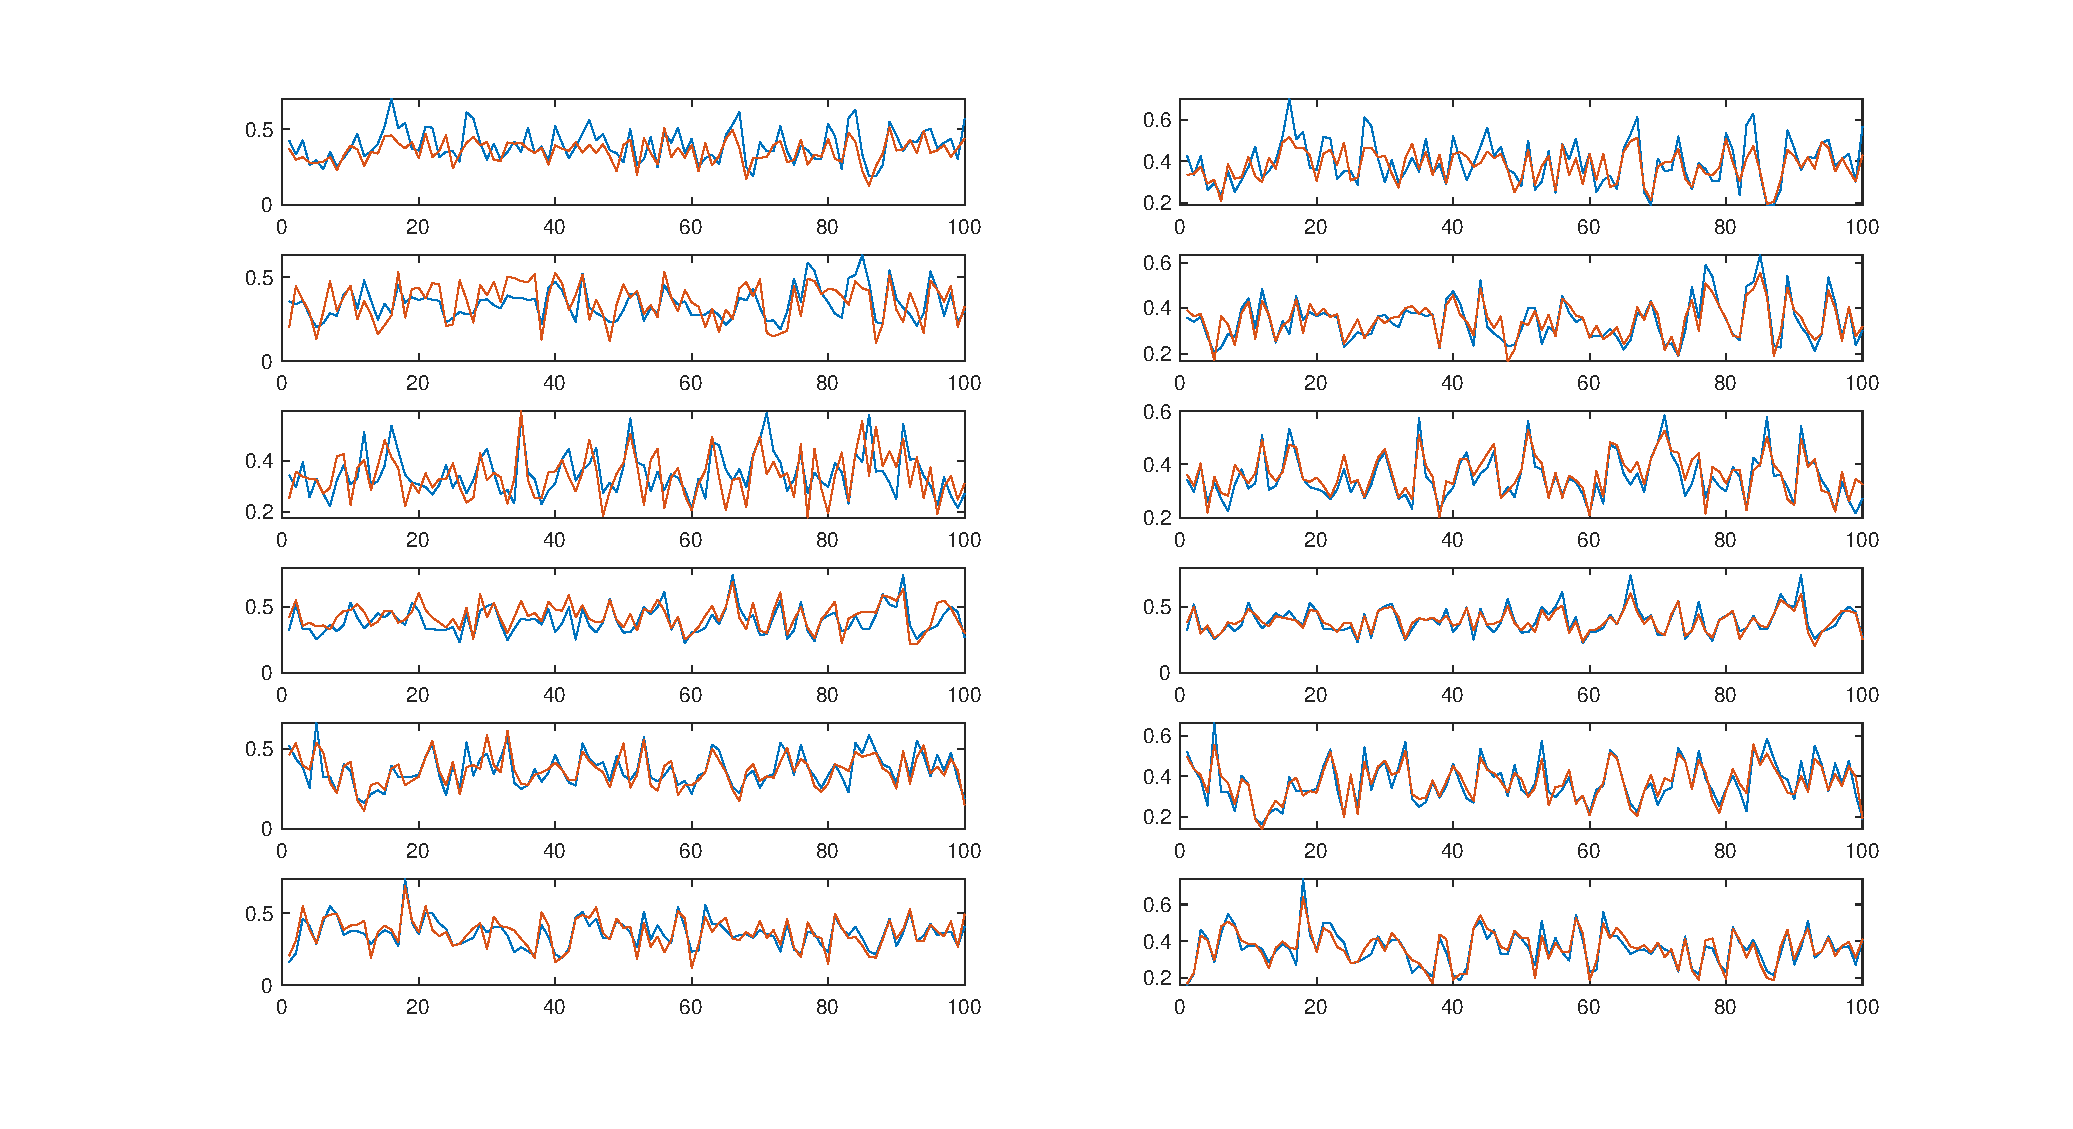
\includegraphics[width=1.0\columnwidth]{exp/fig_accuracy.eps}
%	\caption{accuracy}
%	\label{fig_accuracy}
%\end{figure}
%
%
%\begin{figure}
%	\centering
%	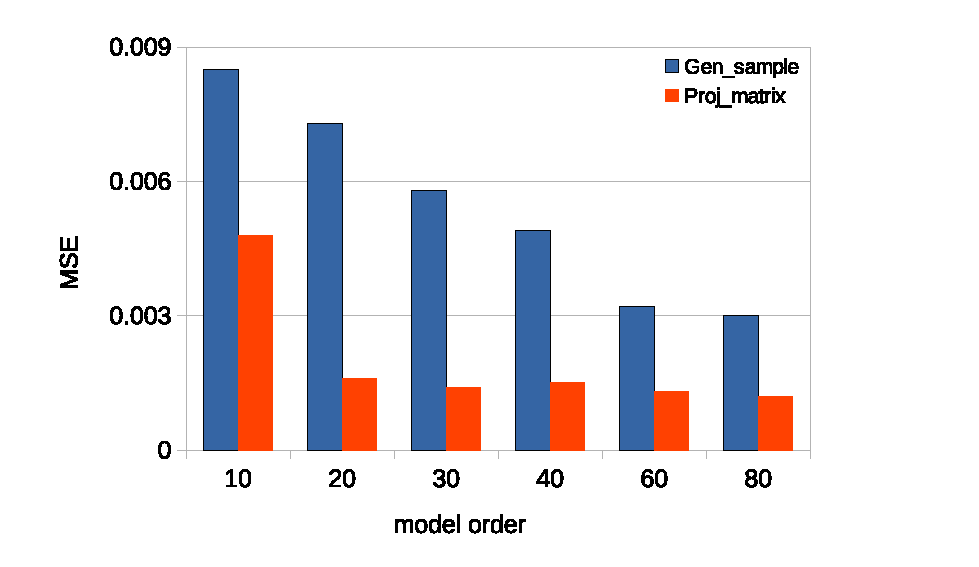
\includegraphics[width=1.0\columnwidth]{exp/chart_accuracy1.eps}
%	\caption{accura}
%	\label{fig_acc}
%\end{figure}
%
%
%
%
%

\begin{tabular}{cccccccc}
\toprule
	 		&		500		&	10		&	20		&	30		&	40		&	60		&	80		\\	\midrule
 Param.		&		26k		&	320		&	1240	&	2760	&	4880	&	10920	&	19360	 \\	\hline
Comp.ratio	&		\#		&	1.2\%	&	4.8\%	&	10.6\%	&	18.8\%	&	42\%	&	74.5\% 	\\	\hline
Time(ms)	&		486121	&	1833		&	2729	&	4093	&	5907	&	10457	&	17031 \\	\hline
Speed up	&		\#		&	265		&	178		&	119		&	82		&	47		&	29 \\	\hline
Perf(FLOPS)	&		534846	&	1745772	&	4543788	&	6743220	&	8261385	&	10442766&	11367506	\\	\hline
Perf.imprv	&		\#		&	3.26	&	8.5		&	12.6	&	15.5	&	19.5	&	21.3	\\
\bottomrule
\end{tabular}



%
%\begin{figure}
%	\centering
%	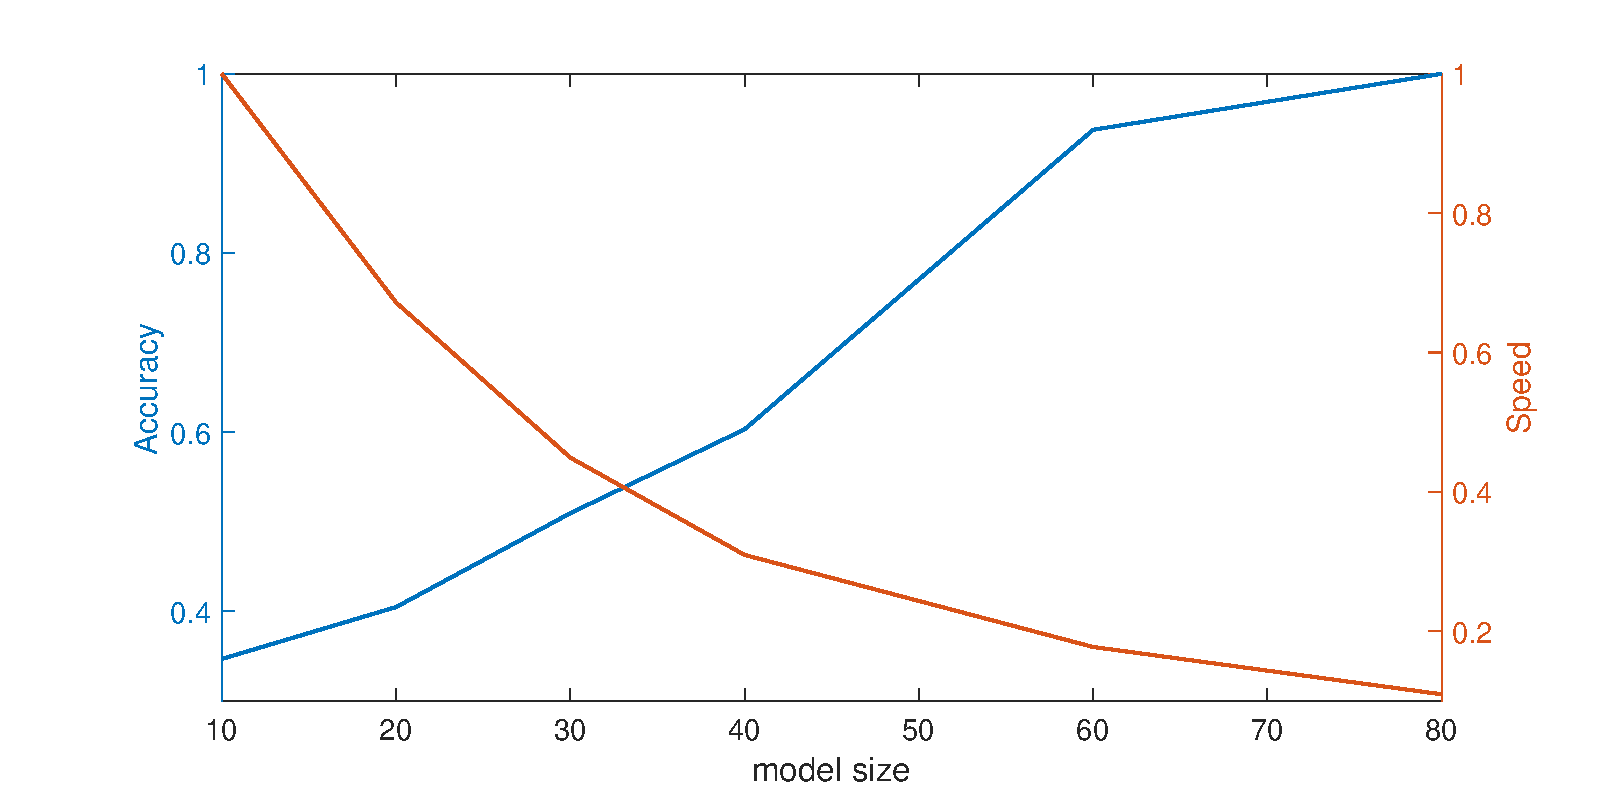
\includegraphics[width=1.0\columnwidth]{exp/fig_acc&speed.eps}
%	\caption{accspeed}
%	\label{fig_accu&speed}
%\end{figure}
%
%
%
%\begin{center}
\begin{table}
\caption{SOC和加速器的资源消耗}
\renewcommand\arraystretch{1.1} 
\setlength{\tabcolsep}{6pt}{
	\begin{tabular}{ccccccc}
	\toprule
				\multicolumn{2}{c}{Resource}	&	LUT		&	LUTRAM	&	FF		&	BRAM	&	DSP	\\	\hline
 								&	Avili.	&	63400	&	19000	&	126800	&	270		&	240 \\	\hline
	\multirow{2}{*}{Accelerator}&	Used	&	21531	&	921	&	41048	&	29	&	66\\
								&	Utili.	&	33.96\%	&	4.85\%	&	32.37\%	&	10.74\%	&	27.59\%	\\
					\hline	
	\multirow{2}{*}{SOC}		&	Used	&	45322	&	5410	&	66090	&	33	&	68\\
								&	Utili.	&	71.49\%	&	28.47\%	&	52.12\%	&	12.22\%	&	28.33\%	\\
	
\bottomrule
\end{tabular}
}
\label{tab:resourceUsed}
\end{table}
\end{center}
\vspace{-3em}



%
